\level{2}{ATimingService}

\level{3}{Structure}
{
\centering{}
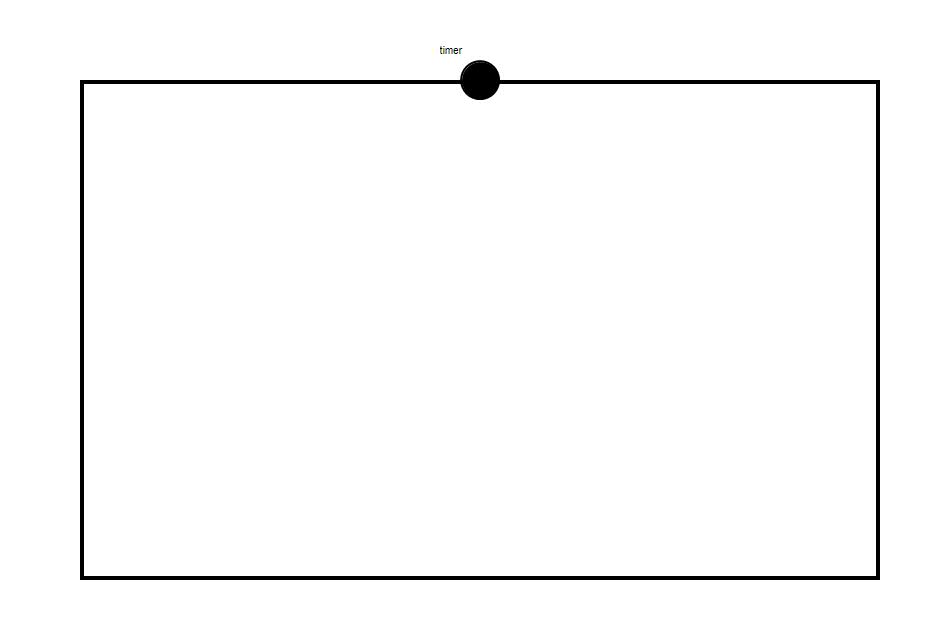
\includegraphics[width=1.0\textwidth]{./images/ATimingService_structure.jpg}
\figcaption{ATimingService Structure}
}


\level{3}{Behavior}
\level{4}{Top Level}
{
\centering{}
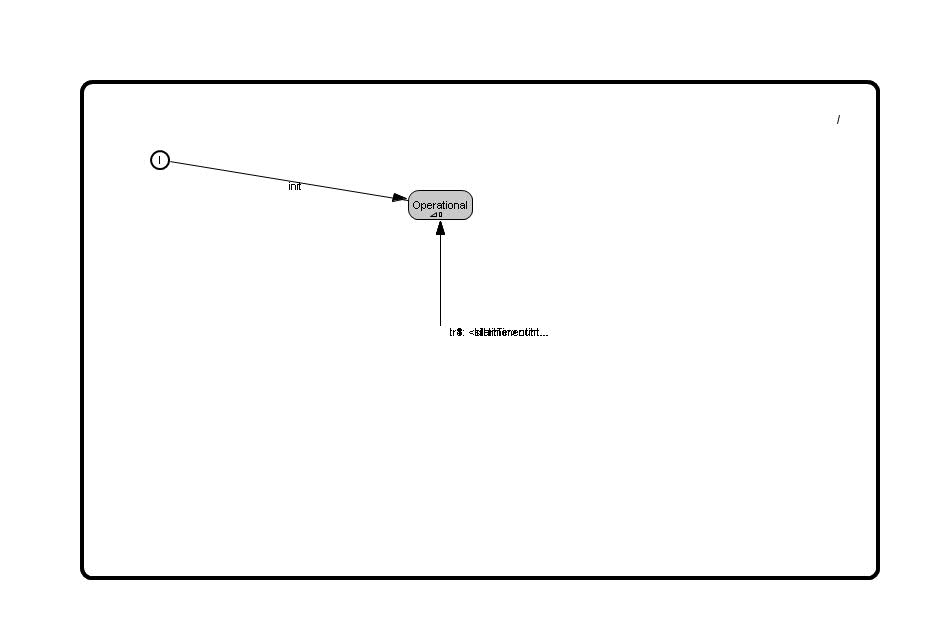
\includegraphics[width=1.0\textwidth]{./images/ATimingService_behavior.jpg}
\figcaption{ATimingService Top State}
}

\begin{par}

\end{par}


\level{3}{Attributes}
\begin{tabular}[ht]{|l|l|p{8cm}|}
\hline
\textbf{Name} & \textbf{Type} & \textbf{Description}\\
\hline
tcbs & tcb & \\
\hline
usedTcbsRoot & tcb & \\
\hline
freeTcbsRoot & tcb & \\
\hline
\end{tabular}

\level{3}{Operations}
\begin{tabular}[ht]{|l|l|}
\hline		
	Name: & getTcb\\
	\hline
	ReturnType: &  tcb\\
	\hline
	Arguments: & \\
	\hline
\end{tabular}
\newline\newline\newline
\begin{tabular}[ht]{|l|l|}
\hline		
	Name: & returnTcb\\
	\hline
	ReturnType: &  void\\
	\hline
	Arguments: & block:tcb\\
	\hline
\end{tabular}
\newline\newline\newline
\begin{tabular}[ht]{|l|l|}
\hline		
	Name: & removeTcbFromUsedList\\
	\hline
	ReturnType: &  void\\
	\hline
	Arguments: & idx:int32\\
	\hline
\end{tabular}
\newline\newline\newline
\begin{tabular}[ht]{|l|l|}
\hline		
	Name: & putTcbToUsedList\\
	\hline
	ReturnType: &  void\\
	\hline
	Arguments: & block:tcb\\
	\hline
\end{tabular}
\newline\newline\newline
\begin{tabular}[ht]{|l|l|}
\hline		
	Name: & isTimeGreater\\
	\hline
	ReturnType: &  boolean\\
	\hline
	Arguments: & t1:targetTime, t2:targetTime\\
	\hline
\end{tabular}
\newline\newline\newline
\begin{tabular}[ht]{|l|l|}
\hline		
	Name: & addTime\\
	\hline
	ReturnType: &  void\\
	\hline
	Arguments: & t1:targetTime, t2:targetTime\\
	\hline
\end{tabular}
\newline\newline\newline
